\documentclass{article}
\usepackage{mathtools,amssymb}
\usepackage{float,graphicx}
\usepackage{nopageno}
\usepackage[letterpaper]{geometry}

\setlength{\parindent}{0in}


\begin{document}

\section*{The Multiplication Principle}

\begin{enumerate}
\item Josh has an orange hat, a blue hat, and a green hat. He has a blue shirt, a green shirt, a red shirt, and a magenta shirt. He also has a pair of red pants and a pair of blue pants. How many different outfits can Josh make that consist of one hat, one shirt, and one pair of pants?\vspace{3cm}
\item How many odd five-digit counting numbers can be formed by choosing digits from the set\par \{1, 2, 3, 4, 5, 6, 7\} if digits \underline{can} be repeated?\vspace{3cm}
\item (2011 National Sprint Problem \#2) A local restaurant boasts that they have 240 different dinner combinations. A dinner combination consists of an appetizer, entree, and dessert. If the restaurant offers 10 appetizer choices and 6 entree choices, how many different dessert choices does it have?\vspace{3cm}
\item A sandwich restaurant offers 6 different meats and 5 different vegetables. For each sandwich, customers can choose at most one meat and up to 5 vegetables. How many different sandwiches does the restaurant offer?
\end{enumerate}


\newpage

\section*{Counting Factors (Divisors)}

\textit{Throughout, only positive factors (divisors) are considered.}

\begin{enumerate}
\item How many factors does 3600 have?\vspace{2cm}
\item (2002 School Sprint Problem \#22) How many odd whole numbers are factors of 180?\vspace{2cm}
\item (2012 National Sprint Problem \#28) How many whole numbers $n$, such that $100\leq n\leq 1000$, have the same number of odd factors as even factors?\vspace{2cm}
\item (2006 State Team) Emma plays with her square unit tiles by arranging all of them into different shaped rectangular figures. (For example, a $5\times 7$ rectangle would use 35 tiles and would be considered the same rectangle as a $7\times 5$ rectangle.) Emma can form exactly ten different such rectangular figures that each use all of her tiles. What is the least number of tiles Emma could have?\vspace{2cm}
\end{enumerate}
\textbf{Additional:} For any real number $k$, the \emph{sum of $k$-th powers of divisors function $\sigma_k$} takes a positive integer $n$ and returns the sum of the $k$-th powers of all divisors of $n$. For example,
\begin{equation*}
\sigma_3(12) = 1^3 + 2^3 + 3^3 + 4^3 + 6^3 + 12^3 = 2044.
\end{equation*}
If $n = p_1^{e_1}p_2^{e_2}\cdots p_r^{e_r}$ is the prime factorization of $n$, then
\begin{equation*}
\boxed{\sigma_k(n) = (1 + p_1^k + p_1^{2k} + \cdots + p_1^{e_1k})(1 + p_2^k + p_2^{2k} + \cdots + p_1^{e_2k})\cdots (1 + p_r^k + p_r^{2k} + \cdots + p_r^{e_rk}).}
\end{equation*}
In our example, $12 = 2^2\cdot 3^1$, so $\sigma_3(12) = (1 + 2^3 + (2^2)^3)(1 + 3^3)$. The most relevant special cases are that $\sigma_0$ is the number-of-divisors function and $\sigma_1$ is the sum-of-divisors function.


\newpage

\begin{enumerate}
\item \underline{\hspace{3in}} (common fraction)\vspace{1cm}
\item \underline{\hspace{3in}}\vspace{1cm}
\item \underline{\hspace{3in}} (in terms of $\pi$)\vspace{1cm}
\item \underline{\hspace{3in}} (in terms of $\pi$)\vspace{1cm}
\item \underline{\hspace{3in}} (in terms of $\pi$)\vspace{1cm}
\item \underline{\hspace{3in}} (in terms of $\pi$)\vspace{1cm}
\item \underline{\hspace{3in}} (simplest radical form)\vspace{1cm}
\item \underline{\hspace{3in}} (in terms of $\pi$, simplest radical form)\vspace{1cm}
\item Each face of a uniform hexagonal prism is to be colored red or blue. In how many ways can this be done if two colorings are considered equivalent whenever one can be rotated to get the other? (A polyhedron is \emph{uniform} if all of its faces are regular polygons.)
\vspace{1cm}
\item In the figure below, lines $\overline{CD}$ and $\overline{EF}$ are tangent to both circles $A$ and $B$. If the radii of the circles are integers, $CD = 12$, and $EF = 10$, then what is $AB$? Express your answer in simplest radical form.
\begin{center}
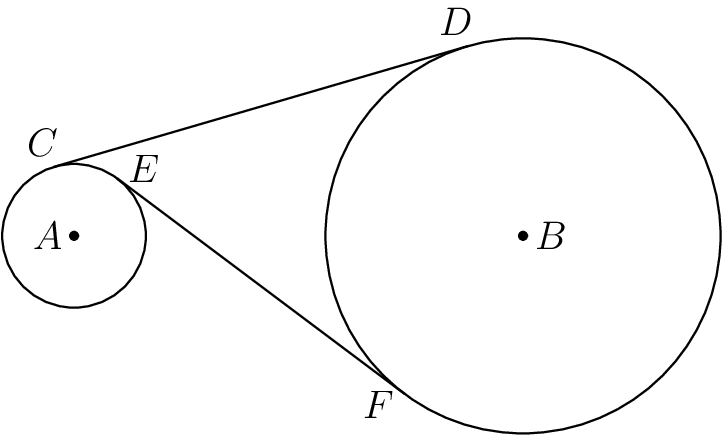
\includegraphics[scale=0.2]{circles.png}
\end{center}
\end{enumerate}


\newpage

\begin{enumerate}
\item $2/3$ (\emph{MATHCOUNTS 2013: School Sprint})\vspace{1cm}
\item $16$ (\emph{MATHCOUNTS 2008: School Team})\vspace{1cm}
\item $26 + 17\pi$ (\emph{MATHCOUNTS 2013: State Countdown})\vspace{1cm}
\item $\pi$\vspace{1cm}
\item $8\pi - 8$ (\emph{MATHCOUNTS 1994: School Team})\vspace{1cm}
\item $8\pi - 16$ (\emph{MATHCOUNTS 1991: National Countdown})\vspace{1cm}
\item $192 + 128\sqrt{3}$\vspace{1cm}
\item $36 - 12\sqrt{3} - 4\pi$ (\emph{MATHCOUNTS 1991: National Team})\vspace{1cm}
\item Each face of a uniform hexagonal prism is to be colored red or blue. In how many ways can this be done if two colorings are considered equivalent whenever one can be rotated to get the other? (A polyhedron is \emph{uniform} if all of its faces are regular polygons.) $\boxed{40}$
\vspace{1cm}
\item In the figure below, lines $\overline{CD}$ and $\overline{EF}$ are tangent to both circles $A$ and $B$. If the radii of the circles are integers, $CD = 12$, and $EF = 10$, then what is $AB$? Express your answer in simplest radical form. $\boxed{2\sqrt{61}}$
\begin{center}
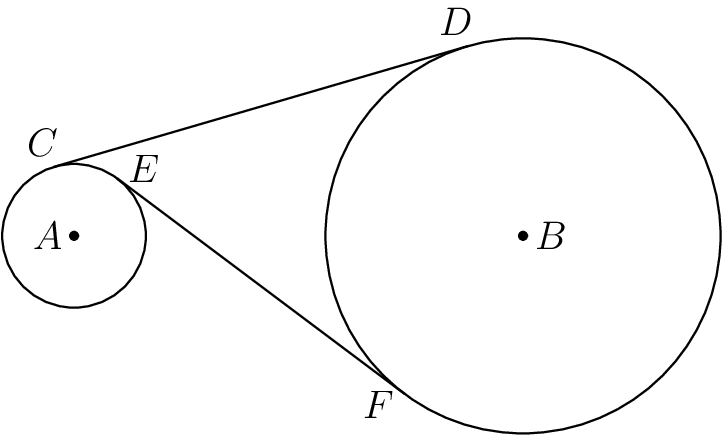
\includegraphics[scale=0.18]{circles.png}
\end{center}
\end{enumerate}

\end{document}

